% Options for packages loaded elsewhere
% Options for packages loaded elsewhere
\PassOptionsToPackage{unicode}{hyperref}
\PassOptionsToPackage{hyphens}{url}
\PassOptionsToPackage{dvipsnames,svgnames,x11names}{xcolor}
%
\documentclass[
  british,
  a4paper,
]{article}
\usepackage{xcolor}
\usepackage{amsmath,amssymb}
\setcounter{secnumdepth}{-\maxdimen} % remove section numbering
\usepackage{iftex}
\ifPDFTeX
  \usepackage[T1]{fontenc}
  \usepackage[utf8]{inputenc}
  \usepackage{textcomp} % provide euro and other symbols
\else % if luatex or xetex
  \usepackage{unicode-math} % this also loads fontspec
  \defaultfontfeatures{Scale=MatchLowercase}
  \defaultfontfeatures[\rmfamily]{Ligatures=TeX,Scale=1}
\fi
\usepackage{lmodern}
\ifPDFTeX\else
  % xetex/luatex font selection
\fi
% Use upquote if available, for straight quotes in verbatim environments
\IfFileExists{upquote.sty}{\usepackage{upquote}}{}
\IfFileExists{microtype.sty}{% use microtype if available
  \usepackage[]{microtype}
  \UseMicrotypeSet[protrusion]{basicmath} % disable protrusion for tt fonts
}{}
\makeatletter
\@ifundefined{KOMAClassName}{% if non-KOMA class
  \IfFileExists{parskip.sty}{%
    \usepackage{parskip}
  }{% else
    \setlength{\parindent}{0pt}
    \setlength{\parskip}{6pt plus 2pt minus 1pt}}
}{% if KOMA class
  \KOMAoptions{parskip=half}}
\makeatother
% Make \paragraph and \subparagraph free-standing
\makeatletter
\ifx\paragraph\undefined\else
  \let\oldparagraph\paragraph
  \renewcommand{\paragraph}{
    \@ifstar
      \xxxParagraphStar
      \xxxParagraphNoStar
  }
  \newcommand{\xxxParagraphStar}[1]{\oldparagraph*{#1}\mbox{}}
  \newcommand{\xxxParagraphNoStar}[1]{\oldparagraph{#1}\mbox{}}
\fi
\ifx\subparagraph\undefined\else
  \let\oldsubparagraph\subparagraph
  \renewcommand{\subparagraph}{
    \@ifstar
      \xxxSubParagraphStar
      \xxxSubParagraphNoStar
  }
  \newcommand{\xxxSubParagraphStar}[1]{\oldsubparagraph*{#1}\mbox{}}
  \newcommand{\xxxSubParagraphNoStar}[1]{\oldsubparagraph{#1}\mbox{}}
\fi
\makeatother


\usepackage{longtable,booktabs,array}
\newcounter{none} % for unnumbered tables
\usepackage{calc} % for calculating minipage widths
% Correct order of tables after \paragraph or \subparagraph
\usepackage{etoolbox}
\makeatletter
\patchcmd\longtable{\par}{\if@noskipsec\mbox{}\fi\par}{}{}
\makeatother
% Allow footnotes in longtable head/foot
\IfFileExists{footnotehyper.sty}{\usepackage{footnotehyper}}{\usepackage{footnote}}
\makesavenoteenv{longtable}
\usepackage{graphicx}
\makeatletter
\newsavebox\pandoc@box
\newcommand*\pandocbounded[1]{% scales image to fit in text height/width
  \sbox\pandoc@box{#1}%
  \Gscale@div\@tempa{\textheight}{\dimexpr\ht\pandoc@box+\dp\pandoc@box\relax}%
  \Gscale@div\@tempb{\linewidth}{\wd\pandoc@box}%
  \ifdim\@tempb\p@<\@tempa\p@\let\@tempa\@tempb\fi% select the smaller of both
  \ifdim\@tempa\p@<\p@\scalebox{\@tempa}{\usebox\pandoc@box}%
  \else\usebox{\pandoc@box}%
  \fi%
}
% Set default figure placement to htbp
\def\fps@figure{htbp}
\makeatother



\ifLuaTeX
\usepackage[bidi=basic,shorthands=off]{babel}
\else
\usepackage[bidi=default,shorthands=off]{babel}
\fi
\ifLuaTeX
  \usepackage{selnolig} % disable illegal ligatures
\fi


\setlength{\emergencystretch}{3em} % prevent overfull lines

\providecommand{\tightlist}{%
  \setlength{\itemsep}{0pt}\setlength{\parskip}{0pt}}



 


\makeatletter
\@ifpackageloaded{tcolorbox}{}{\usepackage[skins,breakable]{tcolorbox}}
\@ifpackageloaded{fontawesome5}{}{\usepackage{fontawesome5}}
\definecolor{quarto-callout-color}{HTML}{909090}
\definecolor{quarto-callout-note-color}{HTML}{0758E5}
\definecolor{quarto-callout-important-color}{HTML}{CC1914}
\definecolor{quarto-callout-warning-color}{HTML}{EB9113}
\definecolor{quarto-callout-tip-color}{HTML}{00A047}
\definecolor{quarto-callout-caution-color}{HTML}{FC5300}
\definecolor{quarto-callout-color-frame}{HTML}{acacac}
\definecolor{quarto-callout-note-color-frame}{HTML}{4582ec}
\definecolor{quarto-callout-important-color-frame}{HTML}{d9534f}
\definecolor{quarto-callout-warning-color-frame}{HTML}{f0ad4e}
\definecolor{quarto-callout-tip-color-frame}{HTML}{02b875}
\definecolor{quarto-callout-caution-color-frame}{HTML}{fd7e14}
\makeatother
\makeatletter
\@ifpackageloaded{caption}{}{\usepackage{caption}}
\AtBeginDocument{%
\ifdefined\contentsname
  \renewcommand*\contentsname{Table of contents}
\else
  \newcommand\contentsname{Table of contents}
\fi
\ifdefined\listfigurename
  \renewcommand*\listfigurename{List of Figures}
\else
  \newcommand\listfigurename{List of Figures}
\fi
\ifdefined\listtablename
  \renewcommand*\listtablename{List of Tables}
\else
  \newcommand\listtablename{List of Tables}
\fi
\ifdefined\figurename
  \renewcommand*\figurename{Figure}
\else
  \newcommand\figurename{Figure}
\fi
\ifdefined\tablename
  \renewcommand*\tablename{Table}
\else
  \newcommand\tablename{Table}
\fi
}
\@ifpackageloaded{float}{}{\usepackage{float}}
\floatstyle{ruled}
\@ifundefined{c@chapter}{\newfloat{codelisting}{h}{lop}}{\newfloat{codelisting}{h}{lop}[chapter]}
\floatname{codelisting}{Listing}
\newcommand*\listoflistings{\listof{codelisting}{List of Listings}}
\makeatother
\makeatletter
\makeatother
\makeatletter
\@ifpackageloaded{caption}{}{\usepackage{caption}}
\@ifpackageloaded{subcaption}{}{\usepackage{subcaption}}
\makeatother
\usepackage{bookmark}
\IfFileExists{xurl.sty}{\usepackage{xurl}}{} % add URL line breaks if available
\urlstyle{same}
% fallback for those not using the hyperref driver hyperxmp:
\makeatletter
\@ifundefined{xmpquote}{\newcommand{\xmpquote}[1]{#1}}{}
\makeatother
\hypersetup{
  pdftitle={Where a funding shock lands: one projection model for advanced and emerging economies},
  pdfauthor={Carlos Galindo},
  pdflang={en-GB},
  colorlinks=true,
  linkcolor={blue},
  filecolor={Maroon},
  citecolor={Blue},
  urlcolor={Blue},
  pdfcreator={LaTeX via pandoc}}


\title{Where a funding shock lands: one projection model for advanced
and emerging economies}
\usepackage{etoolbox}
\makeatletter
\providecommand{\subtitle}[1]{% add subtitle to \maketitle
  \apptocmd{\@title}{\par {\large #1 \par}}{}{}
}
\makeatother
\subtitle{A calibrated quarterly projection model in which the currency
of public and bank debt decides whether stress reaches the exchange rate
or long-dated bond yields, applied to five advanced economies}
\author{Carlos Galindo}
\date{}
\begin{document}
\maketitle


\begin{tcolorbox}[enhanced jigsaw, arc=.35mm, bottomrule=.15mm, breakable, colback=white, colframe=quarto-callout-note-color-frame, left=2mm, leftrule=.75mm, opacityback=0, rightrule=.15mm, toprule=.15mm]

\vspace{-3mm}\textbf{At a glance}\vspace{3mm}

\begin{itemize}
\tightlist
\item
  \textbf{Question.} Can one macroeconomic model read an emerging market
  and an advanced economy alike, without treating every country with a
  deficit as the same case?
\item
  \textbf{Approach.} A calibrated quarterly projection model with a
  regime switch keyed to the currency of public and bank debt, a policy
  rate reserved for inflation and the output gap, and political
  credibility and capital flows acting through risk premia; codified as
  one written specification run under a common evidence standard.
\item
  \textbf{Finding.} The currency of the debt decides where a funding
  shock lands: on the exchange rate where debt is in foreign currency,
  on long-dated government bond yields where it is in local currency.
  Applied to five advanced economies, the readings locate the common
  pressure point in the marginal buyer of long-dated government debt,
  not in headline deficits or currency risk.
\item
  \textbf{Why it matters.} The same deficit headline carries different
  risks in different economies. A model that knows which price can break
  tells an analyst which market to watch, and which signals to discount.
\end{itemize}

\end{tcolorbox}

\subsection{The question}\label{the-question}

Models of small open economies grew up around emerging markets, where
funding stress tends to end in the currency: debt is owed in foreign
currency, reserves run down and the exchange rate gives way. Advanced
economies mostly borrow in their own currency, yet when one runs a
fiscal and an external deficit together it is often read through the
same lens, and the currency is expected to break. That reading runs
together objects that behave differently: the headline current account
and the gap that actually needs financing, the debt ratio and this
year's borrowing, the expected path of the policy rate and the premium
investors charge to hold long-dated bonds.

The question was how to write one model that serves both kinds of
economy, so that a brief on an emerging market and a brief on an
advanced economy use the same equations and differ only where the
economics differs. A second question followed. If the model is applied
across many countries, by different analysts and by different AI models,
what makes two briefs on two economies comparable line by line?

\subsection{Approach}\label{approach}

\textbf{The core.} The starting point is a quarterly projection model in
the form used by the IMF for small open economies, and the work
generalises the central-European scenario framework into a single model.
The output gap depends on expected output and on the real interest rate;
inflation on expected inflation, the output gap, and import and energy
prices; the policy rate on inflation and the output gap; the exchange
rate on interest parity plus a risk premium. The coefficients are
calibration priors, not estimated elasticities: they fix the direction
and rough size of each channel, so the model organises evidence rather
than forecasting from fitted values.

\textbf{Three generalisations.}

\emph{The policy rate does one job.} It reacts to inflation and the
output gap only. Political credibility and capital-flow pressure act
through risk premia on government bonds and on the currency, not through
the policy rule. Credibility is slow and is graded in ordered steps,
each tied to a named event such as a fiscal rule, a budget or an
election, rather than given a continuous score it cannot support. Flow
pressure is fast and is read from a short dashboard of market series,
each kept in its own units rather than added into an index whose parts
do not share a scale.

\emph{Demand responds to the long rate.} Spending depends on the long
real interest rate, and the long-dated yield is split into the expected
path of the policy rate and a term premium measured against a named
decomposition. Energy and import prices enter the inflation equation and
the term premium enters the demand equation, so each shock reaches the
economy through one door.

\emph{The currency of the debt decides which stock can break.} A regime
switch keyed to the currency of public and bank debt chooses the stock
that enters the risk premium. Where debt is owed in foreign currency, a
funding stop can become a currency event, and the objects to watch are
reserve cover and external repayments. Where debt is in local currency,
a stop is a strike by buyers of long-dated government bonds, and the
objects are maturity and the marginal buyer; reserves and gross external
debt are not solvency measures there, and the external stock that
matters is the net international investment position. Where an economy
carries both books, both blocks run side by side and are read
separately, never averaged.

\textbf{One specification, one evidence standard.} The framework is
codified as a single written specification that different AI models
execute. It fixes the order of sources: the central bank, the statistics
office, the debt office and the finance ministry first, international
institutions after them. Every figure is graded established, inferred or
not identified. Where two sources disagree, both are set side by side
and the one used is named; a clause that cannot be sourced is dropped.
The specification fixes the outputs too: a framework section, a dated
snapshot, scenarios that each carry a mechanism and a falsifier, and a
watch-list whose thresholds are stated in the units of the series they
watch.

\subsection{What the work shows}\label{what-the-work-shows}

\textbf{The regime fork.} The first figure runs one funding shock
through both regimes. With foreign-currency debt the shock lands on the
exchange rate and long-dated yields move little; with local-currency
debt the same shock lands on long-dated yields and the currency moves
little. Neither regime is simply safer: each has a different price that
can break, and different things to watch.

\begin{figure}

\centering{

\pandocbounded{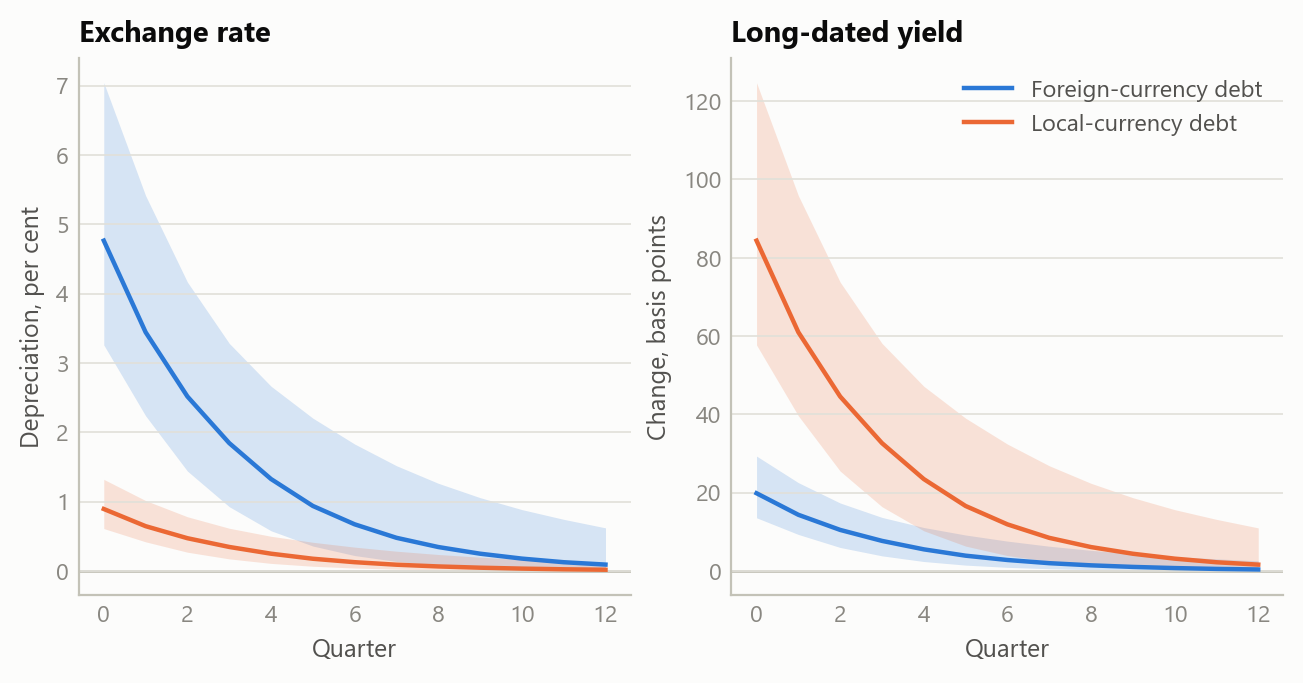
\includegraphics[keepaspectratio]{index_files/figure-latex/fig-fork-output-1.png}}

}

\caption{\label{fig-fork}One funding shock under two debt regimes:
median response and 90\% band of the exchange rate and of the long-dated
yield over twelve quarters (simulated data).}

\end{figure}%

\textbf{A yield rise has two parts.} Once the long rate is split into
path and premium, two episodes with the same rise in yields can mean
different things. When most of a rise is a higher expected path, the
market is pricing the central bank, not refusing the bond, and the
evidence for a buyers' strike sits in the premium alone. The second
figure shows that split for six simulated episodes.

\begin{figure}

\centering{

\pandocbounded{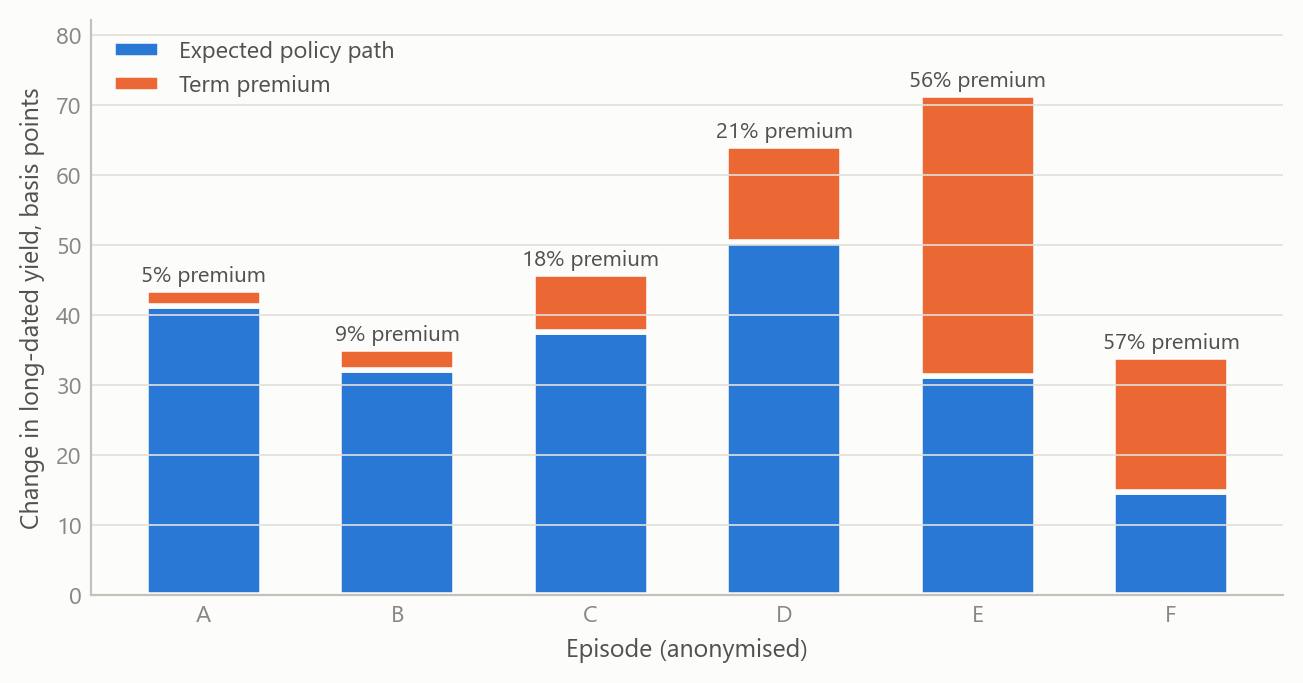
\includegraphics[keepaspectratio]{index_files/figure-latex/fig-split-output-1.png}}

}

\caption{\label{fig-split}Quarterly change in a long-dated yield split
into the expected policy path and the term premium, six episodes ordered
by the premium's share (simulated data).}

\end{figure}%

\textbf{Stock and flow.} The model keeps the debt ratio and the year's
borrowing apart because they answer different questions. A debt ratio
can fall while borrowing runs ahead of the official forecast: that is a
supply question for the next auctions, not a solvency question. The same
separation applies to the external accounts. The headline current
account can include volatile items such as precious metals and
investment income; the gap that needs financing is the underlying one.

\textbf{Five advanced economies.} In October 2026 the specification was
applied to the United States, the United Kingdom, Germany, France and
Japan. All five borrow in their own currency or in one they share, so
all five sit on the local-currency path, and none of the five readings
pointed to a currency stop. For the two euro-area members the policy
rate is set for the union as a whole, so the country-level object for
France is its bond spread over Germany, while Germany, as the benchmark
issuer, has no spread over itself to read. Across the five, the readings
converged on one pressure point: the marginal buyer of long-dated
government debt, rather than the size of the headline deficit or the
external balance. The synthesis therefore ranks the five not by their
deficits but on three questions: whether the debt ratio is rising or
falling, whether long-dated auctions are absorbed, and whether
short-dated yields have already moved away from the policy rate. Where
the evidence for one of these was not published, the readings record it
as not identified rather than filling the gap.

The third figure shows the shape of the cross-country test this reading
implies, on simulated data. If the marginal buyer is the pressure point,
changes in term premia should line up with how well long-dated auctions
are absorbed, and much less with headline deficits.

\begin{figure}

\centering{

\pandocbounded{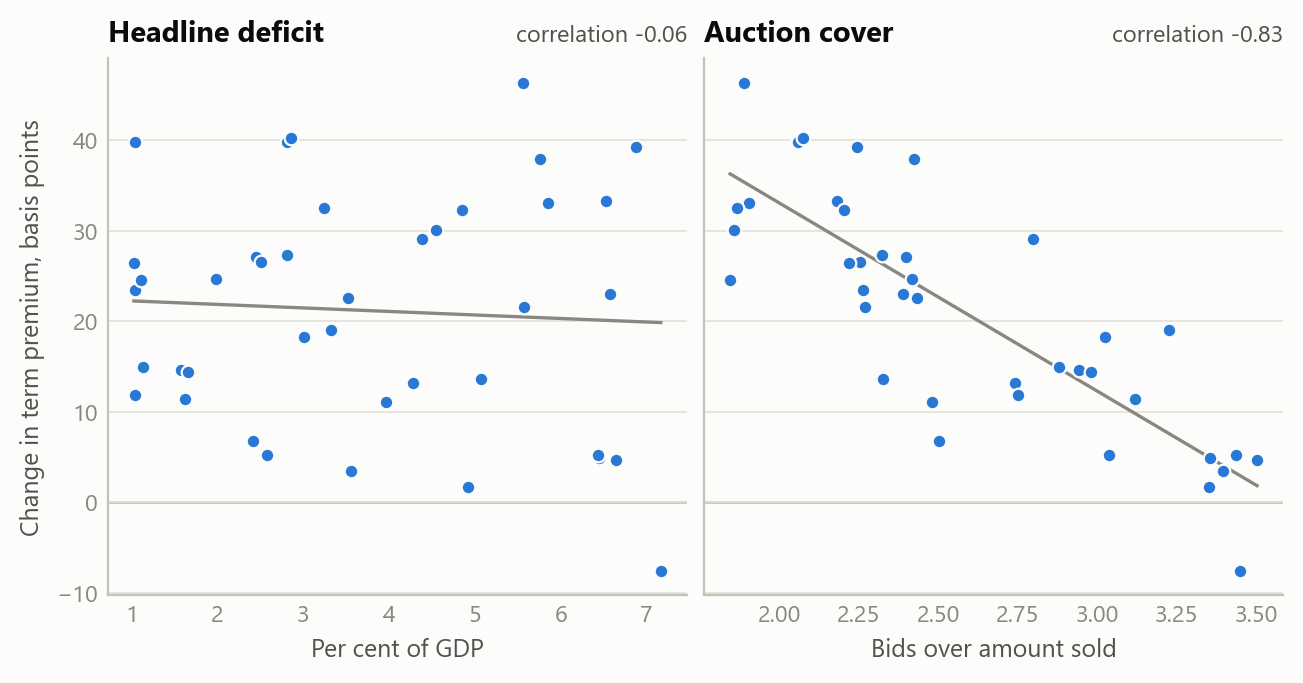
\includegraphics[keepaspectratio]{index_files/figure-latex/fig-buyer-output-1.png}}

}

\caption{\label{fig-buyer}The cross-country test the framework implies:
change in the term premium against the headline deficit and against
auction cover, forty economy-quarters (simulated data).}

\end{figure}%

\subsection{Insights}\label{insights}

\begin{enumerate}
\def\labelenumi{\arabic{enumi}.}
\tightlist
\item
  \textbf{Ask which price can move before asking how far.} The currency
  of the debt decides whether stress lands on the exchange rate or on
  long-dated bonds. A model that settles that first reads an advanced
  economy and an emerging market with the same equations and still tells
  them apart.
\item
  \textbf{Keep the policy rule for inflation and the output gap.}
  Sending credibility and capital flows through risk premia, rather than
  through the policy rate, keeps each channel in one place, where it can
  be seen and tested on its own.
\item
  \textbf{Stock and flow are different questions.} A falling debt ratio
  and a borrowing overrun can coexist; one is about solvency, the other
  about the supply the market must absorb next.
\item
  \textbf{Only the premium part of a yield rise speaks about buyers.} A
  move driven by a higher expected policy path is the market pricing the
  central bank. A buyers' strike shows up in the premium, which has to
  be measured against a named decomposition rather than assumed.
\item
  \textbf{A common evidence standard makes analysis comparable.} When
  every figure carries a grade and every conflict is shown rather than
  averaged, briefs on different economies, written by different models,
  can be read side by side, and a gap in the evidence shows as a gap.
\end{enumerate}

\subsection{Scope and next steps}\label{scope-and-next-steps}

The framework is built to read an advanced economy and an emerging
market with one calibrated model, differing only where the currency of
the debt says they should, and to apply it under an evidence standard
that keeps every figure graded and every conflict in view.

The natural extensions are three. First, the five-economy comparison
tracked through time, with each figure re-read at its official source at
every update. Second, the same specification applied to emerging markets
that borrow in foreign currency and to hybrid cases, where both blocks
run at once. Third, a cross-country test on real data of whether auction
absorption and non-resident take-up explain moves in term premia better
than headline deficits do.

The full specification and the five country readings can be discussed on
request.

\subsection{About the evidence}\label{about-the-evidence}

The work was done in 2026. It rests on a written model specification, a
study of the regime fork on one advanced economy, and a cross-country
synthesis of the five readings, dated October 2026. The coefficients are
calibration priors, not estimates. The market and fiscal figures behind
the readings are not reproduced here. The three figures are simulated,
built to share the structure of the analysis (a quarterly horizon, two
debt regimes, a path-and-premium split of the long yield); none shows a
real estimate.

Figures and tables marked \emph{simulated} are generated from simulated
data built to share the structure of the analysis (its variables,
horizons and frequencies). They show how each method works and what its
output looks like. Results stated in the text, and figures that give a
source, are the project's own. Methods are described at the level of a
methods section. Code and data pipelines are not reproduced here.




\end{document}
